\documentclass{article}

%Page format
\usepackage[table]{xcolor}
\usepackage{pdfpages}
\usepackage{fancyhdr}
\usepackage[margin=1in]{geometry}
\usepackage{tabularx}
%Math packages and custom commands
\usepackage{algpseudocode}
\usepackage{amsthm}
\usepackage{framed}
\usepackage[margin=1in]{geometry}
\usepackage{hyperref}
\usepackage{tikz}
\usepackage[utf8]{inputenc}
\definecolor{Gray}{gray}{0.9}
\usepackage{wrapfig}
\usepackage[margin=1in]{geometry}
\usepackage{mathtools,amsthm}
\usepackage{enumitem,amssymb}
\newtheoremstyle{case}{}{}{}{}{}{:}{ }{}
\theoremstyle{case}
\newtheorem{case}{Case}
\DeclareMathOperator{\R}{\mathbb{R}}
\DeclareMathOperator{\E}{\mathbb{E}}
\DeclareMathOperator{\Var}{\text{Var}}
\DeclareMathOperator{\Cov}{\text{Cov}}
\newcommand{\bvec}[1]{\mathbf{#1}}
\renewcommand{\P}{\mathbb{P}}
\newcommand{\norm}[2][2]{\| #2\|_{#1}}

\definecolor{shadecolor}{gray}{0.9}

\theoremstyle{definition}
\newtheorem*{answer}{Answer}
\newcommand{\note}[1]{\medskip \noindent{\textbf{NOTE:} #1}}
\newcommand{\hint}[1]{\medskip \noindent{\textit{HINT:} #1}}
\newcommand{\recall}[1]{\medskip{[\textbf{RECALL:} #1]}}
\newcommand{\motivation}[1]{\medskip \noindent{\textbf{MOTIVATION:} #1}}
\newcommand{\expect}[1]{\medskip \noindent{\fbox{\parbox{0.95 \textwidth}{\medskip \textbf{What we expect:} #1}}}}
\newcommand{\mysolution}[1]{\noindent{\begin{shaded}\textbf{Your Solution:}\ #1 \end{shaded}}}
\newcommand{\TrainLossNew}{\text{TrainLoss}_{new}}
\newcommand{\TrainLossAvg}{\text{TrainLoss}_{avg}}
\newcommand{\TrainLossMax}{\text{TrainLoss}_{max}}
\newcommand{\TrainLossMaxNew}{\text{TrainLossNew}_{max}}
\newcommand{\TrainLossG}{\text{TrainLoss}_g}
\newlist{todolist}{itemize}{2}
\setlist[todolist]{label=$\square$}
\usepackage{pifont}
% use below to modify the size of equations
% usage is as follows: {fontsize}{math text size}{subscript size}{subsubscript size}
% if you wish to change the math font size, modify {math text size}{subscript size}{subsubscript size} for your chosen global font size {fontsize} which is declared at the beginning of the document
\DeclareMathSizes{10}{13}{13}{13}
\DeclareMathSizes{14}{17}{17}{17}
\DeclareMathSizes{12}{15}{15}{15}
\newcommand{\cmark}{\ding{51}}%
\newcommand{\xmark}{\ding{55}}%
\newcommand{\done}{\rlap{$\square$}{\raisebox{2pt}{\large\hspace{1pt}\cmark}}%
\hspace{-2.5pt}}
\newcommand{\wontfix}{\rlap{$\square$}{\large\hspace{1pt}\xmark}}
\graphicspath{ {./images/} }

\title{\textbf{CS221 Spring 2025: Artificial Intelligence:\\ Principles and Techniques} \\Homework 2: Sentiment Analysis}
\date{}

\chead{Sentiment}
\rhead{\today}
\lfoot{}
\cfoot{CS221: Artificial Intelligence: Principles and Techniques --- Spring 2025}
\rfoot{\thepage}
\renewcommand{\headrulewidth}{0.4pt}
\renewcommand{\footrulewidth}{0.4pt}
\pagestyle{fancy}
\setlength{\parindent}{0pt}

\begin{document}

\maketitle

\begin{center}
\begin{tabular}{rl}
SUNet ID: & [your SUNet ID] \\
Name: & [your first and last name] \\
Collaborators: & [list all the people you worked with]
\end{tabular}
\end{center}
\newcolumntype{g}{>{\columncolor{Gray}}c}
\textit{By turning in this assignment, I agree by the Stanford honor code and declare
that all of this is my own work.} \\
% uncomment one of the below lines to make the text larger
\fontsize{12pt}{16pt}\selectfont
% \fontsize{14pt}{18pt}\selectfont
Advice for this homework:
\begin{itemize}
    \item Words are simply strings separated by whitespace. Note that words which only differ in capitalization are considered separate (e.g. great and Great are considered different words).
    \item You might find some useful functions in \texttt{util.py}. Have a look around in there before you start coding.
\end{itemize}
\textbf{Before you get started, please read the Assignments section on the course website thoroughly}.


\section*{Problem 1: Building intuition}

Here are two reviews of \textit{Perfect Blue}, from \href{https://www.rottentomatoes.com/}{Rotten Tomatoes}: \newline

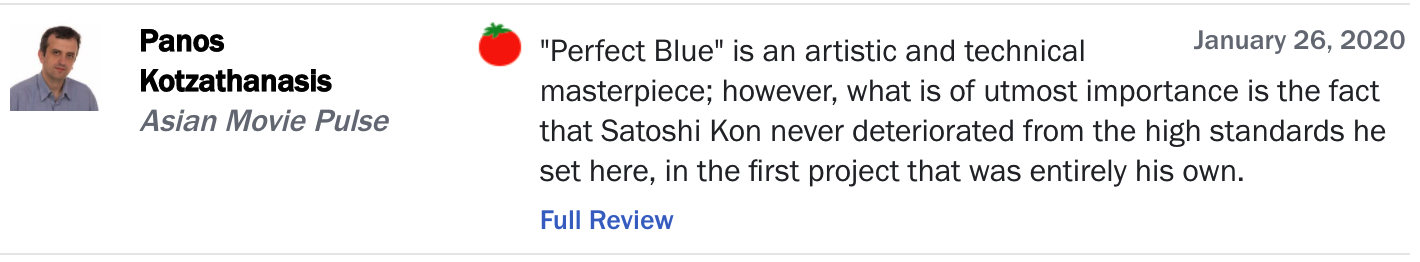
\includegraphics[width=\textwidth]{images/posreview.png}
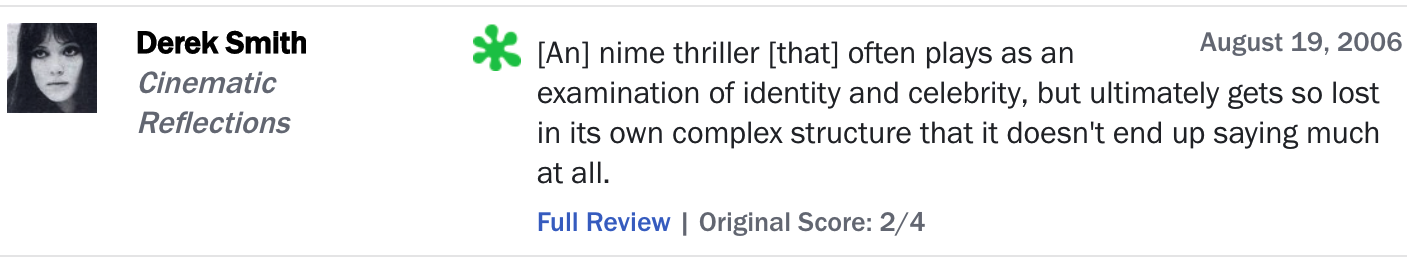
\includegraphics[width=\textwidth]{images/negreview.png}
Rotten Tomatoes has classified these reviews as ``positive" and ``negative,"
     respectively, as indicated by the intact tomato on the top  and the
     splatter on the bottom. In this assignment, you will create a simple
     text classification system that can perform this task automatically. We'll warm up with the following set of four mini-reviews, each labeled
     positive $(+1)$ or negative $(-1)$:
\begin{enumerate}
    \item $(-1)$ not good
    \item $(-1)$ pretty bad
    \item $(+1)$ good plot
    \item $(+1)$ pretty scenery
\end{enumerate}
     Each review $x$ is mapped onto a feature vector $\phi(x)$, which maps each
     word to the number of occurrences of that word in the review. For example,
     the second review maps to the (sparse) feature vector $\phi(x) =
     \{\text{pretty}:1, \text{bad}:1\}$. Recall the definition of the hinge loss:
     $$\text{Loss}_{\text{hinge}}(x, y, \mathbf{w}) = \max \{0, 1 - \mathbf{w}
     \cdot \phi(x) y\},$$ where $x$ is the review text, $y$ is the correct label,
     $\mathbf{w}$ is the weight vector.

\begin{enumerate}[label=\alph*.]
    \item
          $[$2 points$]$ Suppose we run stochastic gradient descent once for each of the 4 samples
       in the order given above, updating the weights according to $$\mathbf{w}
       \leftarrow \mathbf{w} - \eta \nabla_\mathbf{w}
       \text{Loss}_{\text{hinge}}(x, y, \mathbf{w}).$$ After the updates, what
       are the weights of the six words (``pretty", ``good", ``bad", ``plot", ``not",
       ``scenery") that appear in the above reviews?
       \begin{itemize}
           \item Use $\eta = 0.1$ as the step size.
           \item Initialize $\mathbf{w} = [0, 0,0,0,0, 0]$.
           \item The gradient $\nabla_\mathbf{w} \text{Loss}_{\text{hinge}}(x, y,
           \mathbf{w}) = 0$ when margin is exactly 1.
       \end{itemize}
    
    \expect{A weight vector that contains a numerical value for each of the tokens
         in the reviews (``pretty", ``good", ``bad",``plot", ``not", ``scenery"),
         \textbf{in this order}. \\ For example: $[0.1, 0.2,0.3,0.4,0.5, 0.6]$.}
    \mysolution{}
    
    \item $[$2 points$]$
    Given the following dataset of reviews:
\begin{enumerate}[label=\arabic*.]
    \item ($-1$) bad
    \item ($+1$) good
    \item ($+1$) not bad
    \item ($-1$) not good
\end{enumerate}
    Prove that no linear classifier using features of word counts (mapping each word to the number of occurrences of that word in the review) can get zero error on this dataset. Remember that this is a question about classifiers, not
    optimization algorithms; your proof should be true for any linear
    classifier of the form $f_{\mathbf{w}}(x) = \text{sign}(\mathbf{w} \cdot \phi(x))$, regardless of how the weights are learned. 

    Propose a single additional feature for your dataset that we could augment the feature vector with that would fix this problem.
    
    \expect{ 
    \begin{enumerate}[label=\arabic*.]
        \item  A short written proof ($\sim$3-5 sentences).
        \item  A viable feature that would allow a linear classifier to have zero error on the dataset.
    \end{enumerate}
    }
\mysolution{}
\end{enumerate}


\newpage
\section*{Problem 2:  Predicting Movie Ratings}
      Suppose that we are now interested in predicting a numeric rating for
       movie reviews. We will use a non-linear predictor that takes a movie
       review $x$ and returns $\sigma(\mathbf w \cdot \phi(x))$, where $\sigma(z)
       = (1 + e^{-z})^{-1}$ is the logistic function that squashes a real number
       to the range $(0, 1)$. For this problem, assume that the movie rating $y$
       is a real-valued variable in the range $[0, 1]$. \\
       \note{\textbf{Do not} use math software such as Wolfram Alpha to solve this
       problem.}

\begin{enumerate}[label=\alph*.]
    \item $[$2 points$]$
          Suppose that we wish to use
       \textbf{squared loss}. Write out the expression for $\text{Loss}(x, y,
       \mathbf w)$ for a single datapoint $(x,y)$. 
       
       
    \expect{A mathematical expression for the loss. Feel free to use $\sigma$ in the
         expression.}
    \mysolution{}

    \item $[$3 points$]$
   Given $\text{Loss}(x, y, \mathbf w)$ from the previous part, compute the
       gradient of the loss with respect to $\mathbf{w}$, $\nabla_\mathbf{w} \text{Loss}(x, y,
       \mathbf w)$. Write the answer in terms of the predicted value $p =
       \sigma(\mathbf w \cdot \phi(x))$. 
       
    \expect{A mathematical expression for the gradient of the loss.}
    \mysolution{}
    \item $[$3 points$]$
           Suppose there is one datapoint $(x, y)$ with some arbitrary $\phi(x)$ and
       $y = 1$. Specify conditions for $\mathbf w$ to make the magnitude of the
       gradient of the loss with respect to $\mathbf w$ arbitrarily small (i.e.
       minimize the magnitude of the gradient). Can the magnitude of the gradient
       with respect to $\mathbf w$ ever be exactly zero? You are allowed to make
       the magnitude of $\mathbf w$ arbitrarily large but not infinity.
       
       \expect{
       \begin{enumerate}[label=\arabic*.]
           \item 1-2 sentences describing the conditions for $\mathbf w$ to minimize the
         magnitude of the gradient
         \item 1-2 sentences explaining whether the gradient
         can be exactly zero.
       \end{enumerate}} 
         
       \hint{Try to understand intuitively what is going on and what each part
         of the expression contributes. If you find yourself doing too much
         algebra, you're probably doing something suboptimal.}
         
         
                  \motivation{the reason why we're interested in the magnitude of the
         gradients is because it governs how far gradient descent will step. For
         example, if the gradient is close to zero when $\mathbf w$ is very far
         from the optimum, then it could take a long time for gradient descent to
         reach the optimum (if at all). This is known as the
         \textit{vanishing gradient problem} when training neural networks.}
         \mysolution{}

\end{enumerate}


\newpage
\section*{Problem 3: Sentiment Classification}
\begin{wrapfigure}{R}{0.3\textwidth}
\centering

\includegraphics[scale=0.5]{images/sentiment.jpg}
\end{wrapfigure}
In this problem, we will build a binary linear classifier that reads movie reviews and guesses whether they are ``positive" or ``negative.".
   
   
   \note{\textbf{Do not import any outside libraries (e.g. numpy) for any of the coding
     parts.}  Only standard python libraries and/or the libraries imported in the starter
   code are allowed. In this problem, you must implement the functions without
   using libraries like Scikit-learn.

   \hint{look at the provided `util.py` for some helpful utility functions that
   you are able to use when implementing your code. You should use the provided utility methods `dotProduct` and `increment` instead of modifying Python dictionaries directly.}
}

\begin{enumerate}[label=\alph*.]
    \item  $[$2 points$]$ Implement the function \texttt{extractWordFeatures}, which takes a review (string) as input and returns a feature vector
	$\phi(x)$, which is represented as a \texttt{dict} in Python.
	\item $[$4 points$]$ Implement the function \texttt{learnPredictor} using stochastic gradient descent and minimize the hinge loss.
  Print the training error and validation error after each epoch to make sure your code is working.
  You must get less than 4\% error rate on the training set and less than 30\% error rate on the validation set to get full credit.
  \item $[$2 points$]$ Write the \texttt{generateExample} function (nested in the \texttt{generateDataset} function) to generate artificial data samples.
    
    Use this to double check that your \texttt{learnPredictor} works! You can do this by using \texttt{generateDataset()} to generate training and validation examples. You can then pass in these examples as \texttt{trainExamples} and \texttt{validationExamples} respectively to \texttt{learnPredictor} with the identity function \texttt{lambda x:x} as a \texttt{featureExtractor}.
    \item $[$2 points$]$
  Some languages are written without spaces between words.
  So is splitting the words really necessary or can we just naively consider strings of characters that stretch across words?
  Implement the function \texttt{extractCharacterFeatures}
  (by filling in the \texttt{extract} function), which maps each string of $n$ characters to the number of times it occurs, ignoring whitespace (spaces and tabs).
\item $[$3 points$]$
    Run your linear predictor with feature extractor \texttt{extractCharacterFeatures}.  Experiment
    with different values of $n$ to see which one produces the smallest validation error.  You should observe that this error is nearly as small as that produced by word features. Why is this the case? 
    
    Construct a review (one sentence max) in which character $n$-grams probably outperform word features, and briefly explain why this is so.

   \note{There is a function in \texttt{submission.py} that will allow you add a test to \texttt{grader.py} to test different values of $n$. Remember to write your final written solution here. }
   
   \expect{
   \begin{enumerate}[label=\arabic*.]
       \item A short paragraph (~4-6 sentences). In the paragraph state which value of $n$ produces the smallest validation error, why this is likely the value that produces the smallest error.
    \item A one-sentence review and explanation for when character $n$-grams probably outperform word features.
   \end{enumerate}
   }
   \mysolution{}
\end{enumerate}


\newpage
\section*{Problem 4: Toxicity Classification and Maximum Group Loss
}
Recall that models trained (in the standard way) to minimize the average loss can work well on average but poorly on certain groups. One way to mitigate this issue is by minimizing the maximum group loss instead. In this problem, we will compare the average loss and maximum group loss objectives on a toy setting inspired by a problem with real-world toxicity classification models.
\\
\\
Toxicity classifiers are designed to assist in moderating online forums by predicting whether an online comment is toxic or not, so that comments predicted to be toxic can be flagged for humans to review \href{https://web.archive.org/web/20250111062951/https://current.withgoogle.com/the-current/toxicity/}{[1]}.
Unfortunately, some models have been shown to misclassify non-toxic comments mentioning demographic identities (e.g., “I am a [demographic identity]”) as toxic \href{https://medium.com/jigsaw/unintended-bias-and-names-of-frequently-targeted-groups-8e0b81f80a23}{[2]}. This behavior could arise if we assume that toxic comments in the dataset often mention demographic identities, and as a result, models learn to \textit{spuriously correlate} toxicity with the mention of these identities.
 \\
 \\
  In this problem, we will study a toy setting that illustrates the spurious correlation problem:
 The input $x$ is a comment (a string) made on an online forum;
 the label $y \in \{-1,1\}$ is the toxicity of the comment ($y = 1$ is toxic, $y=-1$ is non-toxic);
 $d \in \{0,1\}$ indicates if the text contains a word that refers to a demographic identity;
 and $t \in \{0,1\}$ indicates whether the comment includes certain “toxic” words.
 The comment $x$ is mapped onto the feature vector $\phi(x) = [1, d, t]$ where 1 is the bias term (the bias term is present to  prevent the edge case $ \mathbf{w} \cdot \phi(x) = 0$ in the questions that follow).
 To make this concrete, we provide a few simple examples below, where we underline toxic words and words that refer to a        demographic identity:
 \\
\newline


\begin{tabularx}{1.0\textwidth} { 
  | >{\raggedright\arraybackslash}X 
  | >{\centering\arraybackslash}X 
  | >{\centering\arraybackslash}X 
  | >{\centering\arraybackslash}X | }
 \hline
 \rowcolor{Gray}
 Comment ($x$) &  Toxicity ($y$) & Presence of demographic mentions ($d$) & Presence of toxic words ($t$)  \\
 \hline
 “Stanford \underline{sucks}!” &  1 & 0 & 1 \\
\hline
 “I’m a \underline{woman} in computer science!” & -1 & 1 & 0 \\
 \hline
 “The hummingbird \underline{sucks} nectar from the flower” & -1 & 0 & 1 \\
 \hline
\end{tabularx}
\pagebreak

 Suppose we are given the following training data,
 where we list the number of times each combination $(y, d, t)$ shows up in the training set.
\\

\begin{tabularx}{1.0\textwidth} { 
  | >{\centering\arraybackslash}X 
  | >{\centering\arraybackslash}X 
  | >{\centering\arraybackslash}X 
  | >{\centering\arraybackslash}X | }
 \hline
 \rowcolor{Gray}
 $y$ & $d$ & $t$ & num. examples  \\
 \hline
 -1 & 0 & 0 & 63 \\
\hline
 -1 & 0 & 1 & 27 \\
 \hline
 -1 & 1 & 0 & 7 \\
 \hline
  -1 &	1 &	1 &	3  \\
 \hline
 1 &	0 &	0 &	3  \\
 \hline
  1 &	0 & 	1 &	7 \\
 \hline
  1 & 	1 &	0 &	27 \\
 \hline
  	1 &	1 & 1 & 	63  \\
 \hline
  \multicolumn{3}{|r|}{Total num. examples} &	\textbf{200} \\
  \hline
\end{tabularx}
\\
\\
From the above table, we can see that 70 out of the 100 of toxic comments include toxic words, and 70 out of the 100 non-toxic comments do not. In addition, the toxicity of the comment $y$ is highly correlated with mentions of demographic identities $d$ (again under the assumption that toxic comments target demographic identities) -- 90 out of the 100 toxic comments include mentions of demographic identities, and 90 out of the 100 non-toxic comments do not.
 \\
 \\
   We will consider linear classifiers of the form $f_{\mathbf{w}}(x) = \text{sign}(\mathbf{w} \cdot \phi(x))$, where $\phi(x)$   is defined above.
 Normally, we would train classifiers to minimize either the average loss or the maximum group loss,
 but for simplicity, we will compare two fixed classifiers (which might not minimize either objective):
  \begin{itemize}
      \item Classifier D: $\mathbf{w} = [-0.1, 1, 0]$
      \item Classifier T: $\mathbf{w} = [-0.1, 0, 1]$
  \end{itemize}
   For our loss function, we will be using the zero-one loss, so that the per-group loss is
 $$\text{TrainLoss}_g(\mathbf{w}) = \frac{1}{|\mathcal{D}_\text{train}(g)|}{\sum_{(x,                                           y)\in\mathcal{D}_\text{train}(g)}}\mathbf{1}[f_\mathbf{w}(x)\neq y].$$
 Recall the definition of the maximum group loss:
 $$\text{TrainLoss}_\text{max}(\mathbf{w}) = \max_{g} \text{TrainLoss}_g(\mathbf{w}).$$
 \\
 To capture the spurious correlation problem,
 let us define groups based on the value of $(y, d)$.
 There are thus four groups: $(y=1, d=1), (y=1, d=0), (y=-1, d=1)$, and $(y=-1, d=0)$.
 For example, the group $(y=-1, d=1)$ refers to non-toxic comments with demographic mentions.

\begin{enumerate}[label=\alph*.]
    \item $[$2 points$]$  In words, describe the behavior of Classifier D and Classifier T.
    \\
    \\
    \expect{For each classifier (D and T), an “if-and-only-if” statement describing the output of the classifier in terms of its features when $f_w(x)=1$.}
    \mysolution{}
    \item $[$3 points$]$
    Compute the following three quantities concerning Classifier D using the dataset above:
    \begin{enumerate}[label=\arabic*.]
        \item Classifier D's average loss
        \item Classifier D's average loss for each group (fill in the table below)
        \item Classifier D's maximum group loss
    \end{enumerate}    
    
    \expect{A value for average loss, a complete table (found below) with average loss for each group with the values in the given order, and a value   for maximum group loss.}

\begin{table}[h]
  \centering
    \begin{tabularx}{0.5\textwidth} { 
   | g  
  | >{\centering\arraybackslash}X 
  | >{\centering\arraybackslash}X | }
 \hline
 \rowcolor{Gray}
   Classifier D  & $ y=1$ & $y=-1$ \\
\hline
 $d=1$ & ?? & ?? \\
 \hline
 $d=0$ & ?? & ?? \\
 \hline
\end{tabularx}
  \end{table}
\mysolution{}
\item $[$3 points$]$
Now compute the following three quantities concerning Classifier T using the same dataset:
    \begin{enumerate}[label=\arabic*.]
        \item Classifier T's average loss
        \item Classifier T's average loss for each group (fill in the table below)
        \item Classifier T's maximum group loss
    \end{enumerate}    
Which classifier has lower average loss? Which classifier has lower maximum group loss?
\textbf{Note the groups are still defined by $d$, the demographic label.}

    \expect{A value for average loss, a complete table with average loss for each group with the values in the given order, and a value for maximum group loss. Indicate which classifier has lower average loss, then indicate which classifier has lower maximum group loss.}
    
\begin{table}[h]
  \centering
    \begin{tabularx}{0.5\textwidth} { 
   | g  
  | >{\centering\arraybackslash}X 
  | >{\centering\arraybackslash}X | }
 \hline
 \rowcolor{Gray}
  Classifier T   &  $y=1$ & $y=-1$ \\
\hline
 $d=1$ & ?? & ?? \\
 \hline
 $d=0$ & ?? & ?? \\
 \hline
\end{tabularx}
\end{table}
\mysolution{}
 
\item $[$4 points$]$
As we saw above, different classifiers lead to different numbers of accurate predictions and different people’s comments being wrongly rejected. Accurate classification of a non-toxic comment is good for the commenter, but when no classifier has perfect accuracy, how should the correct classifications be distributed across commenters? 
\\
\\
The module on Algorithms and Distribution \href{https://drive.google.com/file/d/1uwT0rDj47qmB61TvueUlgMdEjmROg6SZ/view}{video}, \href{https://stanford-cs221.github.io/spring2024-extra/modules/machine-learning/algorithms-and-distribution.pdf}{pdf} highlights some well-known principles of fairness distribution (note: reviewing the module will help you answer this question well). These ethical frameworks are a great starting point for thinking through how to choose a classifier, but in reality a combination of approaches might be needed to balance potential trade-offs. 
\\
\\
$\TrainLossNew(w) = \lambda \cdot \TrainLossAvg(w) + (1 - \lambda) \cdot \TrainLossMax(w)$ where $\lambda \in [0,1]$ is a hyperparameter.

\begin{enumerate}[label=\arabic*., wide=0pt]
\item Consider the new loss term above that we want our classifier to minimize. For the case where $\lambda = 1$, describe the optimal classifier according to the ethical frameworks from the module.

\expect{Describe which ethical framework aligns with the optimal classifier in 1-2 sentences. You may reference classifiers D or T when discussing the optimal classifier, but you must justify your answer using the provided ethical framework to earn full points.}
\mysolution{}

\item Now consider the case where $\lambda = 0$, describe the optimal classifier according to the ethical frameworks from the module. 

\expect{Describe which ethical framework aligns with the optimal classifier in 1-2 sentences. You may reference classifiers D or T when discussing the optimal classifier, but you must justify your answer using the provided ethical framework to earn full points.}
\mysolution{}

\item Suppose $\lambda$ is still set to 0. We are given another set of training data, where we list the number of times each combination $(y,d,t)$ shows up in the training set.

\vspace{0.5cm}

\begin{tabularx}{1.0\textwidth} {
| >{\centering\arraybackslash}X
| >{\centering\arraybackslash}X
| >{\centering\arraybackslash}X
| >{\centering\arraybackslash}X | }
\hline
\rowcolor{Gray}
$y$ & $d$ & $t$ & num. examples \\
\hline
-1 & 0 & 0 & 36 \\
\hline
-1 & 0 & 1 & 33 \\
\hline
-1 & 1 & 0 & 32 \\
\hline
-1 & 1 & 1 & 33 \\
\hline
1 & 0 & 0 & 32 \\
\hline
1 & 0 & 1 & 33 \\
\hline
1 & 1 & 0 & 1 \\
\hline
1 & 1 & 1 & 0 \\
\hline
\multicolumn{3}{|r|}{Total num. examples} & \textbf{200} \\
\hline
\end{tabularx}

\vspace{0.5cm}

Let us again define groups based on the value of $(y,d)$. Group $(y=1, d=1)$ has (sample size = 1) and the other three groups have much larger group sizes (group $(y=1, d=0)$ has size 65, group $(y=-1, d=1)$ has size 65, group $(y=-1, d=0)$ has size 69). A valid concern might be that particularly small groups should not be weighted the same as much larger groups of individuals. How would you factor in group size in the $\TrainLossMax(w)$ term to account for this concern? 

Note: There are multiple valid answers to this problem.

\expect{Justify your proposed adjustment to the loss term in 1-2 sentences.}
\mysolution{}

\item What value of $\lambda$ in $\TrainLossNew(w)$ (without the adjustment from the previous part) would you deploy in the following scenario? A real online social media platform is using a classifier to flag posts as toxic for review. The platform cares equally about average loss and minimizing the maximum loss per group. Again, make sure that your argument refers to the ethical frameworks mentioned in the module and discusses the trade-offs. 

\expect{There are many ways to answer these questions well; a good answer explains the connection between a classifier, the loss function and the ethical principle clearly and concisely in 3-5 sentences.}
\mysolution{}
\end{enumerate}
\end{enumerate}
\newpage
\section*{Problem 5: K-means Clustering}
  Suppose we have a feature extractor $\phi$ that produces 2-dimensional feature
   vectors, and a toy dataset $\mathcal D_\text{train} = \{x_1, x_2, x_3, x_4\}$
   with
  \begin{enumerate}
      \item $\phi(x_1) = [0, 0]$
      \item $\phi(x_2) = [4, 0]$
      \item $\phi(x_3) = [6, 0]$
      \item $\phi(x_4) = [11, 0]$
  \end{enumerate}
\begin{enumerate}[label=\alph*.]
    \item $[$2 points$]$
    Run 2-means on this dataset until convergence. Please show your work. What
       are the final cluster assignments $z$ and cluster centers $\mu$? Run this
       algorithm twice with the following initial centers:
       \begin{enumerate}
           \item $\mu_1 = \phi(x_1) = [0, 0]$ and $\mu_2 = \phi(x_4) = [11, 0]$
           \item $\mu_1 = \phi(x_1) = [0, 0]$ and $\mu_2 = \phi(x_2) = [4, 0]$
       \end{enumerate}
       \expect{Show the cluster centers and assignments for each step, and the loss for each final clustering.}
       \mysolution{}
       \item $[$5 points$]$
       Implement the \texttt{kmeans} function. You should initialize your $k$
       cluster centers to random elements of \texttt{examples}.
        After a few iterations of k-means, your centers will be very dense
       vectors. In order for your code to run efficiently and to obtain full
       credit, you will need to precompute certain dot products for squared distance calculation. As a reference,
       our code runs in under a second on cardinal, on all test cases. You might
       find \texttt{generateClusteringExamples}
       in \texttt{util.py} useful for testing your code.
       
       \note{\textbf{Do not} use libraries such as Scikit-learn.}
       
       \item $[$2 points$]$
       In general, if we scale all dimensions in our initial centroids and data points by
       some non-zero factor, are we guaranteed to retrieve the same clusters after running
       k-means (i.e. will the same data points belong to the same cluster before
       and after scaling)? What if we scale only certain dimensions? If your
       answer is yes, provide a short explanation; if not, give a counterexample.
       
       \expect{This response should have two parts. The first should be a yes/no
         response and explanation or counterexample for the first subquestion
         (scaling all dimensions). The second should be a yes/no response and
         explanation or counterexample for the second subquestion (scaling only
         certain dimensions). Note that you should not only consider the above toy dataset, think generally.}
         \mysolution{}
\end{enumerate}
\pagebreak


\section*{Submission}



Submission is done on Gradescope. \\

\textbf{Written:} When submitting the written parts, make sure to select \textbf{all} the pages that contain part of your answer for that problem, or else you will not get credit.
To double check after submission, you can click on each problem link on the right side and it should show the pages that are selected for that problem. \\

\textbf{Programming:} After you submit, the autograder will take a few minutes to run. Check back after it runs to make sure that your submission succeeded. If your autograder crashes, you will receive a 0 on the programming part of the assignment. Note: the only file to be submitted to Gradescope is $\texttt{submission.py}$.\\

More details can be found in the Submission section on the course website.


\end{document}